\documentclass[10pt]{beamer}
\usepackage{graphicx}
\usepackage{adjustbox}

\setbeamertemplate{navigation symbols}{}

\usetheme{Boadilla}
% \setbeamercovered{transparent}
\usecolortheme[named=red]{structure}

\title[Introduction to Agile Software Development]{
  Introduction to Agile Software Development \\
  \vspace{1cm}
  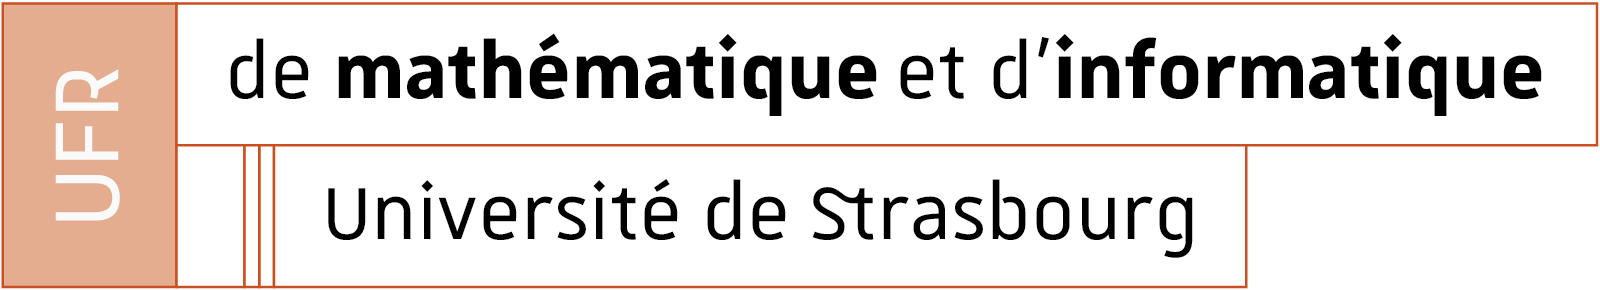
\includegraphics[width=0.6\pdfpagewidth]{images/logo_Uni.png}
}
\author[SuperAgile]{Carpi Lapi, Regardin, Senger, Sengler}
\date[February 7, 2024]{February 7, 2024}

\begin{document}


\frame{\titlepage}

\begin{frame}{What is Agile methodology?}
The Agile methodology is a project management approach that involves:
\begin{itemize}
    \item breaking the project into phases
    \item emphasizes continuous collaboration and improvement \\
    \vspace{1cm}
\end{itemize}

Teams follow a cycle of: 
\begin{itemize}
    \item planning
    \item executing
    \item evaluating
\end{itemize}

\end{frame}


\begin{frame}{Agile vs Waterfall}
  \vspace{0.5cm}
  \adjincludegraphics[height=7cm,trim={0 0 0 0},clip]{images/waterfall_agile.png}
\end{frame}

\begin{frame}{Agile vs Waterfall}
  \vspace{0.5cm}
  \begin{columns}[T]
    \begin{column}{0.5\textwidth}
      \adjincludegraphics[height=10cm,trim={0 0 0 3cm},clip]{images/waterfall.png}
    \end{column}

    \begin{column}{0.5\textwidth}
      \vspace{2cm}
      \begin{itemize}
        \item<2-> Emphasizes detailed upfront \textbf{planning}
        \item<3-> Progress is measured by meeting project \textbf{milestones}
        \item<4-> Rigidity can lead to \textbf{difficulties in responding to changes}
        \item<5-> Suitable for projects with \textbf{well-defined requirements}
      \end{itemize}
    \end{column}
  \end{columns}
\end{frame}

\begin{frame}{Agile vs Waterfall}
  \vspace{2cm}
  \begin{columns}[T]
    \begin{column}{0.5\textwidth}
      \begin{itemize}
        \item<2-> \textbf{Adaptive approach }to changing requirements
        \item<3-> Embraces \textbf{flexibility} and customer collaboration
        \item<4-> \textbf{Iterative} and incremental development
        \item<5-> Customer \textbf{feedback} is incorporated throughout the process
      \end{itemize}
    \end{column}

    \begin{column}{0.5\textwidth}
      \adjincludegraphics[height=10cm,trim={16cm 0 0 7cm},clip]{images/agile.png}
      
    \end{column}
  \end{columns}
\end{frame}


\begin{frame}{General Agile guideline}
    Marie
\end{frame}

\begin{frame}{The Agile Timeline}
    Antoine
\end{frame}

\begin{frame}{Pros and Cons of the Agile Method}
    Antoine
\end{frame}

\begin{frame}{Conclusion}
  
\end{frame}

\begin{frame}{References}

  \begin{itemize}
    \item https://www.youtube.com/watch?v=goJu-DFGJ0o
    \item https://www.youtube.com/watch?v=1evfn3qTYGM
    \item https://project-management.com/agile-project-management/
  \end{itemize}
  
\end{frame}

\end{document}
